
%=================================================================
\ifx\wholebook\relax\else
% --------------------------------------------
% Lulu:
	\documentclass[a4paper,10pt,twoside]{book}
	\usepackage[
		papersize={6.13in,9.21in},
		hmargin={.75in,.75in},
		vmargin={.75in,1in},
		ignoreheadfoot
	]{geometry}
	\input{../common.tex}
	\setboolean{lulu}{true}
% --------------------------------------------
% A4:
%	\documentclass[a4paper,11pt,twoside]{book}
%	\input{../common.tex}
%	\usepackage{a4wide}
% --------------------------------------------
    \graphicspath{{figures/} {../figures/}}
    \DeclareGraphicsExtensions{.png,.jpg,.pdf,.eps,.gif}
	\newcommand{\fig}[4]{
		\begin{figure}[#1]
			\centering
			\includegraphics[width=#2\textwidth]{#3}
			\caption{\label{fig:#3}#4}
		\end{figure}}

	\newcommand{\largefig}[4]{
		\begin{figure*}[#1]
			\centering
			\includegraphics[width=#2\textwidth]{#3}
			\caption{\label{fig:#3}#4}
		\end{figure*}}
		
	\newcommand{\asdf}[4]{
		\begin{subfigure}[\label{fig:#3}]
                \centering
                \includegraphics[width=\textwidth]{#3}
                \caption{\label{fig:#3}#4}                
        \end{subfigure}}

\begin{document}
\fi
%=================================================================
%\renewcommand{\nnbb}[2]{} % Disable editorial comments
\sloppy
%=================================================================
\chapter{Agile Visualization with Roassal}
\chalabel{roassal}


Giving a meaning to a a large amount of data is challenging without adequate tools. Textual outputs are known to be limited in their expression and interactions. 

Roassal is an agile visualization engine. It is made to visualize and interact with any arbitrary data, defined in terms of objects and their relationships. Roassal is commonly employed in producing interacting \vp{interactive?} visualization. Roassal is used by the Moose community to visualize software. This chapter introduces Roassal's principles and describes its expressive commands to quickly render your data. After its reading, you will be able to create interactive and visual representation.

%=====================
\section{Installation and first visualization}

Mondrian is available via a Metacello configuration. Just open a workspace and type:
\ja{we need a stable version before the publishing}
\begin{code}{}
Gofer new
	squeaksource: 'Roassal'; 
	package: 'ConfigurationOfRoassal';
	load.
(Smalltalk at: #ConfigurationOfRoassal) project lastVersion load.
\end{code}


\begin{code}{}
| view |
view := ROMondrianViewBuilder new.
view shape rectangle 
	width:  [ :cls | cls numberOfVariables * 5 ];  
	height: #numberOfMethods;
	linearFillColor: #numberOfLinesOfCode within:  Collection withAllSubclasses.
		
view interaction action: #browse.

view nodes: ROShape withAllSubclasses.
view edgesFrom: #superclass.
view treeLayout.
view open
\end{code}

%=====================

\section{Roassal Core Model}

Each Roassal visualization is an instance of the class \textbf{ROView}, which is the container for all the data to be visualize.
Data is represented by instances of \textbf{ROElement} that will be added to the visualization. The value of the data is stored in its \ct{model} instance variable.

The following code to creates and open a visualization with a simple ROElement, which size its 100:



\begin{figure}[H]
      \begin{minipage}[t]{0.5\textwidth}
      \vspace{0pt}
\begin{code}{}
view := ROView new.
element := 
	ROElement new size: 100.
view add: element.
view open.
\end{code}
   \end{minipage}
   \hfill
   \begin{minipage}[t]{0.6\textwidth}
      \vspace{0pt} \raggedright
       \centering
		\includegraphics[width=0.6\textwidth]{ex1}
   \end{minipage}
\label{fig:ex1}
\end{figure}

However, by executing this code nothing appears in the visualization. The element is there but we haven't set how it should look like. The look of a ROElement is given by shapes, instances of subclasses of the abstract class \textbf{ROShape}. Let's add some shape to our element:

\begin{figure}[H]
      \begin{minipage}[t]{0.5\textwidth}
      \vspace{0pt}
\begin{code}{}
view := ROView new.
element := ROElement new size: 100.
element 
	+ ROBorder. "-> add shape"
view add: element.
view open.
\end{code}
   \end{minipage}
   \hfill
   \begin{minipage}[t]{0.6\textwidth}
      \vspace{0pt} \raggedright
       \centering
		\includegraphics[width=0.6\textwidth]{ex2}
   \end{minipage}
\label{fig:ex2}
\end{figure}

To add a ROShape to an instance of ROElement, we send the \textbf{\#+} message with the ROShape wanted to added. For this example we added the ROBorder shape. As its name suggests, ROBorder adds a border to the ROElement. As default, the color of created border is black. There are several other shapes that can be added and they can even be composed. \secref{shapes} details more on shapes and explains how to create more complex looks.

A ROElement can also have interactions, allowing it to answer to events. For instance, they can be dragged by the mouse. To add an interaction to a ROElement send the \textbf{\#@} message with the interaction as parameter: 

\begin{code}{}
view := ROView new.
element := ROElement new size: 100.
element 
	+ ROBorder; "-> add shape"
	@ RODraggable. "-> add interaction"
view add: element.
view open.
\end{code}

Visualization are usualy composed of more than one data value. You can add more elements to a ROView by sending the message \#addAll: with a collection of ROElements. You can later access them by using the \#elements accessor. 

\begin{figure}[H]
      \begin{minipage}[t]{0.5\textwidth}
      \vspace{0pt}
\begin{code}{}
view := ROView new.
element1 := (ROElement new size: 100).
element2 := (ROElement new size: 50).
view addAll: (Array with: element1 with: element2).
view elements do: [:el | el + ROBorder; @ RODraggable].
view open.
\end{code}
   \end{minipage}
   \hfill
   \begin{minipage}[t]{0.6\textwidth}
      \vspace{0pt} \raggedright
       \centering
		\includegraphics[width=0.6\textwidth]{ex3}
   \end{minipage}
\label{fig:ex3}
\end{figure}

By executing this code a visualization with two elements appears, both placed in the top left part. A ROElement can be translated using the \#translateBy: or \#translateTo: selector.

\begin{figure}[H]
      \begin{minipage}[t]{0.5\textwidth}
      \vspace{0pt}
\begin{code}{}
view := ROView new.
element1 := (ROElement new size: 100).
element2 := (ROElement new size: 50).
element2 translateBy: 150@150.
view addAll: (Array with: element1 with: element2).
view elements do: [:el | el + ROBorder; @ RODraggable].
view open.
\end{code}
   \end{minipage}
   \hfill
   \begin{minipage}[t]{0.6\textwidth}
      \vspace{0pt} \raggedright
       \centering
		\includegraphics[width=0.6\textwidth]{ex4}
   \end{minipage}
\label{fig:ex4}
\end{figure}


When a visualization contains more than one element it is hard to setup each position by hand. Roassal provides defined layouts to arrange ROElement's. Layouts are explained in  \secref{layouts}.

A ROElement can also contain other ROElement's, creating nested elements:

\begin{figure}[H]
      \begin{minipage}[t]{0.5\textwidth}
      \vspace{0pt}
\begin{code}{}
view := ROView new.
parent := ROElement new 
				size: 100;
				+ ROBorder.
children := ROElement new 
				size: 50;
				+ ROBorder red.
parent add: children.
view add: parent.
view open.
\end{code}
   \end{minipage}
   \hfill
   \begin{minipage}[t]{0.6\textwidth}
      \vspace{0pt} \raggedright
       \centering
		\includegraphics[width=0.6\textwidth]{ex5}
   \end{minipage}
\label{fig:ex5}
\end{figure}

\vp{not sure if the camera should be explained here. What can be added here about the camera that helps you to build a visualization?}
Another important component of a ROView is the camera, represented by an instance of a \textbf{ROCamera}. A ROCamera is the point of view from which a view object is actually viewed.

\subsubsection*{The Collection hierarchy example}
\vp{I am not sure if this is the right order of if I will not add color}
As an example we will visualize the Collection hierarchy through the chapter. We will build it by executing the following steps:
\begin{enumerate}
\item Add all the data with no particular shape. In this case: Collection with all its subclasses;
\item make the classes look according to metrics of each them;
\item add links between a class and its superclass;
\item arrange the elements as an hierarchy with a layout.
\end{enumerate}

In this section, we start with the first step: adding all the data:
\begin{figure}[H]
\begin{code}{}
view := ROView new.
classes := ROElement forCollection: Collection withAllSubclasses.
classes 
	do: [:c | c + ROBorder.
			c @RODraggable ].
view addAll: classes.
ROHorizontalLineLayout new on: view elements.
view open.
\end{code}
\end{figure}

\fig{H}{0.6}{hier1}{Adding the data}

The \#forCollection: selector of ROElement is just a helper to build ROElement's more easily from a collection. Each resulting ROElement represents each element of the collection parameter. We make them draggable to be more easy to manipulate.
Finally to identify each element easily, we apply a default layout. More explanation of how layouts works will be explained later on. 

%\alex{Describe the core of Roassal: Element, shape, view and camera. We should simply use ``ROElement new'', no need to mention \#on: for now}
%
%\alex{We need to find a small example that we enhance in the chapter. Maybe a System complexity built by hand (ie. without the Mondrian builder).}


%=====================
\section{More on Shapes} \seclabel{shapes}

A ROElement can be shaped by sending the \textbf{\#+} message to an instance of a ROShape or to a ROShape class. When sending to the class, the element is shaped with default values for each attribute.

Some of the shapes available in Roassal are ROLabel, ROBorder, ROBox and ROCircle. By default, \textbf{ROLabel} will display the data of the element associated as string, but it is also possible to set a custom text (\figref{label}). When applying \textbf{ROBorder}, \textbf{ROBox} and \textbf{ROCircle} to a ROElement, the shape will be adapted to the bounds of the element. It is also possible to set attributes as color, border color o border width to a shape. This is shown in \figref{border}, \figref{box} and \figref{circle}.

\begin{figure}[H]
      \begin{minipage}[t]{0.5\textwidth}
      \vspace{0pt}
     \begin{code}
     
	ROElement new 
		size: 100; 
		+ (ROLabel text: 'hello!').	\end{code}
   \end{minipage}
   \hfill
   \begin{minipage}[t]{0.4\textwidth}
      \vspace{0pt} \raggedright
       \centering
		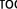
\includegraphics[width=0.4\textwidth]{label}
   \end{minipage}
\caption{ROLabel}
\label{fig:label}
\end{figure}

\begin{figure}[H]
      \begin{minipage}[t]{0.5\textwidth}
      \vspace{0pt}
     \begin{code}
     
	ROElement new 
		size: 100; 
		+ ROBorder.	\end{code}
   \end{minipage}
   \hfill
   \begin{minipage}[t]{0.4\textwidth}
      \vspace{0pt} \raggedright
       \centering
		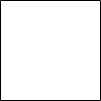
\includegraphics[width=0.25\textwidth]{border}
   \end{minipage}
\caption{ROBorder}
\label{fig:border}
\end{figure}  

\begin{figure}[H]
      \begin{minipage}[t]{0.5\textwidth}
      \vspace{0pt}
     \begin{code}
     
ROElement new 
	size: 200; 
	+ (ROBox new 
				color: Color green; 
				borderColor: Color red; 
				borderWidth: 4 ).	\end{code}
   \end{minipage}
   \hfill
   \begin{minipage}[t]{0.4\textwidth}
      \vspace{0pt} \raggedright
       \centering
		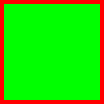
\includegraphics[width=0.5\textwidth]{box}
   \end{minipage}
\caption{ROBox}
\label{fig:box}
\end{figure} 

\begin{figure}[H]
      \begin{minipage}[t]{0.5\textwidth}
      \vspace{0pt}
     \begin{code}
     
ROElement new 
	size: 100; 
	+ (ROCircle new 
				color: Color yellow; 
				borderColor: Color blue; 
				borderWidth: 2 ).	\end{code}
   \end{minipage}
   \hfill
   \begin{minipage}[t]{0.4\textwidth}
      \vspace{0pt} \raggedright
       \centering
		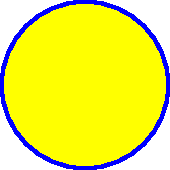
\includegraphics[width=0.25\textwidth]{circle}     
   \end{minipage}
\caption{ROCircle}
\label{fig:circle}
\end{figure}

To create more complex looks we can compose shapes. To have an element shaped with more than one ROShape, we send the \textbf{\#+} message several times with the desired shapes (\figref{composed}). This builds a chain of shapes associated to the element.

\begin{figure}[H]
      \begin{minipage}[t]{0.5\textwidth}
      \vspace{0pt}
     \begin{code}
     
ROElement new 
	size: 180;  
	+ (ROLabel new text: 'composed shape');
	+ (ROBorder new color: Color red); 
	+ (ROCircle new color: Color yellow; 
					borderWidth: 0 ).	\end{code}
   \end{minipage}
   \hfill
   \begin{minipage}[t]{0.4\textwidth}
      \vspace{0pt} \raggedright
       \centering
		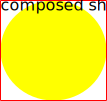
\includegraphics[width=0.4\textwidth]{composed}
   \end{minipage}
\caption{Composing shapes}
\label{fig:composed}
\end{figure} 

\subsubsection*{The Collection hierarchy example}
We now will add some shape to the \ct{Collection} example. Each element representing a class will have a width according to the number of instance variables of the class and a height according to the number of its methods. Like this we are applying metrics to have a polymetric representation of the class.

\begin{code}{}
view := ROView new.
classes := ROElement forCollection: Collection withAllSubclasses.
classes do: [:c | 
	c width: c model instVarNames size.
	c height: c model methods size.
	c + ROBorder. 
	c @ RODraggable ].
view addAll: classes.
ROHorizontalLineLayout new on: view elements.
view open.
\end{code}

\fig{H}{0.6}{hier2}{Adding some shape for each class}


%=====================
\section{Edges: linking elements} \seclabel{edges}

In Roassal it is possible to build links between elements to represent relationships between them. A link between elements is an instance of the class \textbf{ROEdge}. An edge needs two elements: one to be the starting point and another to be the end point. It is important to notice than an edge also needs to be shaped. The following code shows a very simple example of how to build an edge between two ROElement's.


\begin{figure}[H]
 \begin{code}{}
view := ROView new.
fromElement := (ROElement on: 1) size:20; + ROBorder red.
toElement := (ROElement on: 2)  size:20; + ROBorder red.
toElement translateBy: 50@50.

edge := ROEdge from: fromElement to: toElement.
edge + ROLine new. "-> an edge needs to be shaped too"
view 
	add: fromElement; 
	add: toElement; 
	add: edge. "-> and added to the visualization"
view inspect.
\end{code}   
\caption{Simple edge}
\label{fig:simpleEdge}
\end{figure} 

There are several ways to shape a ROEdge. Some examples are shown in \figref{line}, \figref{arrowEdge} and \figref{orthoEdge}.

\begin{figure}[H]
      \begin{minipage}[t]{0.5\textwidth}
      \vspace{0pt}
     \begin{code}{}
edge + ROLine new. \end{code}
   \end{minipage}
   \hfill
   \begin{minipage}[t]{0.4\textwidth}
      \vspace{0pt} \raggedright
       \centering
		\includegraphics[width=0.4\textwidth]{line}
   \end{minipage}
\caption{Simple edge}
\label{fig:line}
\end{figure} 

\begin{figure}[H]
      \begin{minipage}[t]{0.5\textwidth}
      \vspace{0pt}
     \begin{code}{}
edge + (ROLine new add: ROArrow new). \end{code}
   \end{minipage}
   \hfill
   \begin{minipage}[t]{0.4\textwidth}
      \vspace{0pt} \raggedright
       \centering
		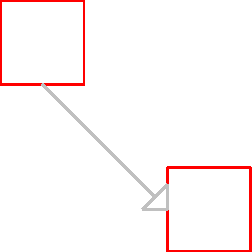
\includegraphics[width=0.4\textwidth]{arrowEdge}
   \end{minipage}
\caption{Arrowed edge}
\label{fig:arrowEdge}
\end{figure} 

\begin{figure}[H]
      \begin{minipage}[t]{0.5\textwidth}
      \vspace{0pt}
     \begin{code}{}
edge + (ROOrthoHorizontalLineShape new add: ROHorizontalArrow new)\end{code}
   \end{minipage}
   \hfill
   \begin{minipage}[t]{0.4\textwidth}
      \vspace{0pt} \raggedright
       \centering
		\includegraphics[width=0.4\textwidth]{orthoEdge}
   \end{minipage}
\caption{Orthogonal edge with horizontal oriented arrow}
\label{fig:orthoEdge}
\end{figure} 

\subsubsection*{The Collection hierarchy example}
Now we know how to make links between elements. With the following code we can create edges between each class to its superclass. To do so, we first need to create a collection of associations of the elements in our view. Each association represents the starting point of the ROEdge to create as the association key and the ending point as the association value. For this example each association goes from a ROElement representing a class to a ROElement that represents its superclass. After having the associations we create the instances of ROEdge by using the \#linesFor: selector.

\begin{code}{}
view := ROView new.
classes := ROElement forCollection: Collection withAllSubclasses.
classes do: [:c | 
	c width: c model instVarNames size.
	c height: c model methods size.
	c + ROBorder. 
	c @ RODraggable ].
view addAll: classes.
associations := classes 
					collect: [:c | 	(c model superclass = Object)
										ifFalse: [ (view elementFromModel: c model superclass) -> c]]
					thenSelect: [:assoc | assoc isNil not ].
edges := ROEdge linesFor: associations.
view addAll: edges.
ROHorizontalLineLayout new on: view elements.
view open
\end{code}

\fig{H}{0.6}{hier3}{Adding links between each class and its superclass}

Now we have each class in the \ct{Collection} hierarchy with the shape we want and connected with each superclass. However we don't see a real hierarchy. This is because we need an appropriate layout to arrange all the elements of the view. Next section covers how to apply layouts to elements.


%=====================
\section{More on Layouts} \seclabel{layouts}
A layout defines how a collection of ROElement can be arranged automatically. Layouts inherits from the \textbf{ROLayout} class. To apply  layout use the \#on: selector with a collection of ROElement's, as shown in \figref{ROGrid}.


\begin{figure}[H]
      \begin{minipage}[t]{0.5\textwidth}
      \vspace{0pt}
     \begin{code}{}
view := ROView new.
view 
	addAll: (ROElement spritesOn: (1 to: 4)).
ROGridLayout on: view elements.
view open.
  \end{code}
   \end{minipage}
   \hfill
   \begin{minipage}[t]{0.6\textwidth}
      \vspace{0pt} \raggedright
       \centering
		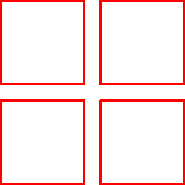
\includegraphics[width=0.3\textwidth]{ROGrid} %layout1?
   \end{minipage}
\label{fig:ROGrid}
\caption{ROGridLayout applied to a group of ROElements}
\end{figure} 

The selector \#spriteOn: creates a collection of ROElement's, each with size 50, shaped with a red border and draggables.

Some of the layouts available in Roassal can be seen in \figref{roLayouts}.

\begin{figure} [H]
        \centering
		\subfigure[ROGridLayout]{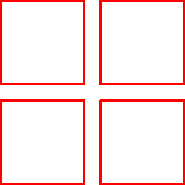
\includegraphics[width=0.15\textwidth]{ROGrid}} \hfill
		\subfigure[ROCircleLayout]{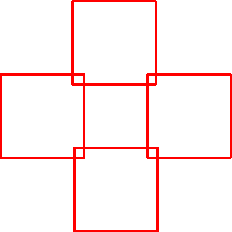
\includegraphics[width=0.15\textwidth]{ROCircle}}\hfill
		\subfigure[ROTreeLayout]{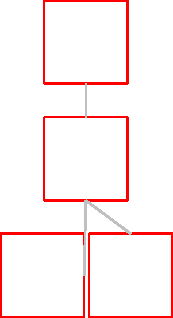
\includegraphics[width=0.11\textwidth]{ROTree}} \\ 
		\subfigure[ROMapTreeLayout]{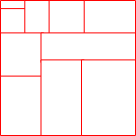
\includegraphics[width=0.2\textwidth]{ROMapTree}} \hfill
		\subfigure[ROVerticalLineLayout]{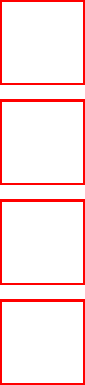
\includegraphics[width=0.06\textwidth]{ROVertical}}\hfill
		\subfigure[ROHorizontalLineLayout]{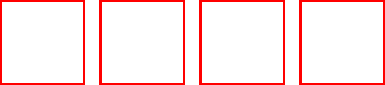
\includegraphics[width=0.25\textwidth]{ROHorizontal}}
        \caption{Some of the layouts availables in Roassal applied to a group of ROElement's}\label{fig:roLayouts}
\end{figure}

When dealing with nested ROElement's, layouts can be relative to each element container.

\begin{figure}[H]
      \begin{minipage}[t]{0.61\textwidth}
      \vspace{0pt}
     \begin{code}{}
view := ROView new.
elements := (ROElement spritesOn: (1 to: 2)).
elements 
	do: [:el | el addAll: (ROElement spritesOn: (1 to: 3)). 
			   ROGridLayout on: el elements.].			   
view addAll: elements.
ROHorizontalLineLayout on: view elements.
view open.
  \end{code}
   \end{minipage}
   \hfill
   \begin{minipage}[t]{0.6\textwidth}
      \vspace{0pt} \raggedright
       \centering
		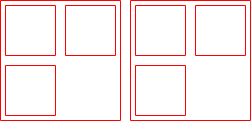
\includegraphics[width=0.6\textwidth]{nestedLayout}
   \end{minipage}
\label{fig:nestedLayout}
\caption{Nested elements with different layouts }
\end{figure} 

\subsubsection*{The Collection hierarchy example}
As we need an hierarchy, the \textbf{ROTreeLayout} will be useful to obtain the Collection hierarchy.
\begin{figure}[H]
\begin{code}{}
view := ROView new.
classes := ROElement forCollection: Collection withAllSubclasses.
classes do: [:c | 
	c width: c model instVarNames size.
	c height: c model methods size.
	c + ROBorder. 
	c @ RODraggable ].
view addAll: classes.
associations := classes collect: [:c | 
	(c model superclass = Object)
		ifFalse: [ (view elementFromModel: c model superclass) -> c]
	 ] thenSelect: [:assoc | assoc isNil not ].
edges := ROEdge linesFor: associations.
view addAll: edges.
ROTreeLayout new on: view elements.
view open
\end{code}
\end{figure}

We did it! :) \vp{<-ok, maybe remove this} The resulting visualization can be seen in \figref{collectionHierarchy}.

\fig{H}{0.4}{collectionHierarchy}{Collection class hierarchy}

%=====================

\section{Events and Callbacks}

Roassal allows any visible component in a visualization, including itself, to react to events. There are two kind of events defined in Roassal. In the first kind are those responding to external events, like mouse clicks, mouse move o key pressing. The second kind of events includes all those triggered by internal manipulation of the ROView or its components, like when a view needs to be refreshed.
All events inherits from the \textbf{ROEvent} class.

There are several event classes to deal with mouse events: \textbf{ROMouseClick}, \textbf{ROMouseMove}, \textbf{ROMouseEnter} and \textbf{ROMouseLeave}, among others; and to deal with key pressing, the \textbf{ROKeyDown} class.

To see how events work, we will make a visualization to react to mouse clicks, translating its only element to where the click was made. For this, we make the visualization to react to ROLeftMouseClick. The reaction will create an animation to translate the element to the event position.

\begin{figure}[H]
      \begin{minipage}[t]{0.61\textwidth}
      \vspace{0pt}
     \begin{code}{}
view := ROView new.
el := ROElement sprite.
view add: el.
view 
	on: ROMouseLeftClick 
	do: [ :event | 
		ROLinearMove new
			for: el to: event position.
	].
view open.
  \end{code}
   \end{minipage}
   \hfill
\caption{Move a ROElement by a ROMouseLeftClick event on its view }
\end{figure} 

\textbf{ROLinearMove} belongs to the Roassal interactions. As its name suggest, makes an animation for an element to be translated in a linear move. More about interactions are explained in next section.

%
%\alex{How to define callbacks}
%\alex{What are the different events we can handle}


%=====================
\section{The Interaction hierarchy}

As previously presented, a ROElement can respond to events by adding interactions to it. The root class of all Roassal interactions is \textbf{ROInteraction}.

There are interactions that makes elements to react to events, such as \textbf{RODraggable}, that allows an element to be dragged by the mouse, or \textbf{ROGrowable}, that makes an element to increase its size when clicked. Some of this interactions can be more complex like popups elements, accesible by the subclasses of \textbf{ROAbstractPopup}, which are displayed when the mouse is over an element. 

Animations are also interactions in Roassal. Some animations allows elements to be translated, like \textbf{ROLinearMove}. \textbf{ROZoomInMove} and \textbf{ROZoomOutMove} allow the view to be zoomed in or out, respectively. All animations are subclasses of \textbf{ROAnimation}.

From the availables interactions in Roassal, two examples are presented: \textbf{ROAbstractPopup} and \textbf{ROAnimation}.

\subsubsection*{ROAbstractPopup}

ROAbstractPopup allows elements to react to mouse over events by displaying a popup. There are two kind of popups, (i) \textbf{ROPopup}, which by default displays a box with the String of the value of the ROElement; and (ii) \textbf{ROPopupView}, that displays a custom view.

To add a popup to an element just send the \#@ selector with the ROPopup class. It is also possible to setup a custom text using the \#text: selector with the custom String.

\begin{figure}[H]
      \begin{minipage}[t]{1\textwidth}
      \vspace{0pt}
     \begin{code}{}
view := ROView new.
el := ROElement spriteOn: 'Roassal'.
el @ ROPopup. "Or with custom text -> (ROPopup text: 'this is custom text')"
view add: el.
view open.
  \end{code}
   \end{minipage}
   \hfill
   \begin{minipage}[t]{1\textwidth}
	 \vspace{0pt} \raggedright
       \centering
		\includegraphics[width=0.7\textwidth]{popup}
   \end{minipage}
\label{fig:popup}
\caption{ROPopup}
\end{figure} 

ROPopupView is slightly more complex as it needs the view to popup definition. This interaction can be created by sending the \#view: selector to the \textbf{ROPopupView} class with the view to be displayed. The parameter can also be a block with one parameter, which will be evaluated with the element where the interaction belongs to.

\begin{figure}[H]
      \begin{minipage}[t]{1\textwidth}
      \vspace{0pt}
     \begin{code}{}
view := ROView new.
elements := ROElement spritesOn: (1 to: 5).
"create the view to popup"
viewToPopup :=
	[:el |
		|v| 
		v := ROView new.
		v addAll: (ROElement forCollection: (1 to: el model )).
		v elementsDo: [:e | e size: 20; + ROBox ].
		ROGridLayout on: v elements.
		v].
elements 
	do: [:e | e + ROLabel; 
				@ (ROPopupView view: viewToPopup)].
view addAll: elements.
ROHorizontalLineLayout on: view elements.
view open.
  \end{code}
   \end{minipage}
   \hfill
   \begin{minipage}[t]{1\textwidth}
	 \vspace{0pt} \raggedright
       \centering
		\includegraphics[width=0.7\textwidth]{popupView2}
   \end{minipage}
\label{fig:popupView}
\caption{ROPopupView}
\end{figure} 


%first example
%view := ROView new.
%el := ROElement spriteOn: 'Roassal'.
%
%"create the view to popup"
%viewToPopup := ROView new.
%viewToPopup 
%	addAll: (ROElement forCollection: (1 to: 4 )).
%viewToPopup 
%	elementsDo: [:e | e size: 20. e + ROBox  ].
%ROGridLayout 
%	on: viewToPopup elements.
%	
%el := ROElement spriteOn: 'Roassal'.
%el @ (ROPopupView view: viewToPopup).
%view add: el.
%view open.


%
%\vp{not sure if present this one}
%\subsubsection*{ROMenuActivable}
%
%\begin{figure}[H]
%      \begin{minipage}[t]{1\textwidth}
%      \vspace{0pt}
%     \begin{code}{}
%view := ROView new.
%el := ROElement sprite.
%el @ (ROMenuActivable new item: 'inspect' action: #inspect).
%view add: el.
%view open.
%  \end{code}
%   \end{minipage}
%   \hfill
%   \begin{minipage}[t]{1\textwidth}
%	 \vspace{0pt} \raggedright
%       \centering
%		\includegraphics[width=0.7\textwidth]{menuActivable}
%   \end{minipage}
%\label{fig:menuActivable}
%\caption{ROMenuActivable applied to a ROElement}
%\end{figure} 

\subsubsection*{ROAnimation}

\vp{working here!}
An animation is as a set of .
By
It also allows to set a block to be executed after the animation is finished, using the \#after: selector. It is important to notice that any action to be done when the animation is finished must be set before the animation is triggered, otherwise it will not be executed.


\alex{Present the hierarchy of the interaction}

\alex{Give some examples with buttons and animations}


%=====================
\section{More on Camera}

\alex{MiniMap}
\alex{Semantic zooming: Making objects appear when the camera goes down}




%=====================
\section{The Mondrian DSL}

How the builder works

%=====================
\section{Beyond Pharo}

Roassal has been ported to VisualWorks, Amber, VA Smalltalk.

\alex{Describe the platform architecture}

%=====================

\section{Conclusion}

Roassal enables any graph of objects to be visualized. This chapter has reviewed the main features of Roassal:
\begin{itemize}
\item blah1
\item blah2
\end{itemize}

\paragraph{Acknowledgment}
We are very grateful to Nicolas Rosselot Urrejola for his review of an early draft of the chapter.

%Mondrian is a perpetual evolving application. This chapter intents to cover the features frequently used. If there is a topic you wish to see discussed here, send an email to alexandre@bergel.eu.
%
%We hope you haved enjoyed it!
%
%=====================


%=============================================================
\ifx\wholebook\relax\else
   \bibliographystyle{jurabib}
   \nobibliography{scg}
   \end{document}
\fi
%=============================================================


%Dead text:

Node color \ja{nothing about edge color ? I think we can say that it is possible too} is an important information support, as the width and the height of a node. Color should be easy to pick to represent particular condition.

The keyword if:fillColor: enables one to assign a color for a particular condition. Consider we want to extend the previous example by coloring abstract classes in red.

\begin{code}{}
view shape rectangle
  width: [ :each | each instVarNames size * 3 ];
  height: [ :each | each methods size ];
  if: #isAbstractClass fillColor: Color red.
view nodes: Collection withAllSubclasses.

view edges: Collection withAllSubclasses from: #yourself toAll: #subclasses.

view treeLayout.
\end{code}


The message \ct{if:fillColor:} may be sent to a shape to conditionally set a color. \ja{what is the link with the source code below ?}

\begin{code}{}
view shape rectangle
  width: [ :each | each instVarNames size * 3];
  height: [ :each | each methods size ];
  if: #isAbstractClass fillColor: Color red.
view nodes: Collection withAllSubclasses.

view edgesFrom: #superclass.

view treeLayout.
\end{code}

All red nodes represent abstract class. Waving the moose above a node make a text tooltip appear revealing its name. 

\ja{it should not be here, we are in section 'adding colors'}
Extended possibilities exist to define interaction. We will review them in a future section. For now, if you are interested in opening a system browser directly from a node, you define this interaction: \ja{can you display only the line concerned ? it is difficult to read each time the same code with only one line changed}

\begin{code}{}
view interaction action: #browse.
view shape rectangle
  width: [ :each | each instVarNames size * 3];
  height: [ :each | each methods size ];
  if: #isAbstractClass fillColor: Color red.
view nodes: Collection withAllSubclasses.

view edgesFrom: #superclass.

view treeLayout.
\end{code}

You can easily \ja{I think there are too much 'easy' or 'easily' in the chapter} spot some red node that do not have subclasses. This indicates a design flow since an abstract must to have subclasses. It makes no sense for a class that is not supposed to be instantiated (since it is abstract) to not have a subclass.

The very same analyzes can be realized on your own classes.

\ja{is this code useful ? it seems to be the same as above}

\begin{code}{}
view interaction action: #browse.
view shape rectangle
  width: [ :each | each instVarNames size * 3];
  height: [ :each | each methods size ];
  if: #isAbstractClass fillColor: Color red.
view nodes: (PackageInfo named: 'Mondrian') classes.

view edgesFrom: #superclass.

view treeLayout.
\end{code}

A shape may contains more than one condition. Let's distinguish abstract classes from classes that define abstract methods.

\begin{code}{}
view shape rectangle
  width: [ :each | each instVarNames size * 3];
  height: [ :each | each methods size ];
  if: #isAbstractClass fillColor: Color lightRed;
  if: [:cls | cls methods anySatisfy: #isAbstract ] fillColor: Color red.

view nodes: Collection withAllSubclasses.

view edgesFrom: #superclass.

view treeLayout.
\end{code}

All red nodes are still abstract classes. Light red indicates classes that do not define abstract methods; strong red indicates classes that define at least one abstract method.

%-----------------------------------------------------------------

%%% Local Variables:
%%% coding: utf-8
%%% mode: latex
%%% TeX-master: t
%%% TeX-PDF-mode: t
%%% ispell-local-dictionary: "english"
%%% End:
